\documentclass[12pt, a4paper]{article}
\usepackage[russian]{babel}
\usepackage[utf8]{inputenc}
\usepackage[T2A]{fontenc}
\usepackage{amsfonts}
\usepackage{amsmath}
\usepackage[
left 	= 	30	mm,
right 	=	15	mm,
top 	=	20	mm,
bottom 	=	20	mm,
]{geometry}

\usepackage{indentfirst} % Красная строка

\setlength{\parindent}{1.25 cm}

\usepackage[toc,page]{appendix}

\renewcommand{\baselinestretch}{1.5}

\usepackage{titlesec}

\titleformat{\section}
{\normalfont\fontsize{14}{14}\bfseries}{\thesection}{1em}{}

\titleformat{\subsection}
{\normalfont\fontsize{14}{14}\bfseries}{\thesubsection}{1em}{}

\usepackage[intoc]{nomencl}
\renewcommand{\nomname}{Обозначения и сокращения}
\makenomenclature

%%% Математика

% Шрифты для математики
\usepackage{amsmath}
\usepackage{amsfonts}
\usepackage{amssymb}
\usepackage{cancel}
\usepackage{mathrsfs}
\usepackage{mathtools}
\usepackage{upgreek}
\usepackage{xfrac}


%%% Иллюстрации
\usepackage{graphicx}
\usepackage{subcaption}
\usepackage{wrapfig}
\usepackage[export]{adjustbox}
%\graphicspath{{./img/}}

\makeatletter % список литературы
\def\@biblabel#1{#1. }
\makeatother

% Графики
\usepackage{pgfplots}
\pgfplotsset{compat=1.3}
\usepgfplotslibrary{patchplots}
%\usepackage{patchplots}
\pgfplotsset{	width	=	14	cm,
	x label style={
		font = {\small\sffamily},
		yshift = 1mm
	},
	tick label style={
		font = {\scriptsize},
	},
	y label style={
		font = {\small\sffamily},
		yshift = -1mm,
		at={(ticklabel cs:0.5)},
		%      					rotate=90,
		anchor=near ticklabel
	},
	every tick/.style	=	{
		black, 
		line width 	= 	.5	pt
	},
	axis line style 	= 	{
		line width 	= 	.5	pt
	},
	grid style	=	{
		gray,
		dotted
	},
	minor x tick num = 1,
	minor y tick num = 1,
	no markers,
	grid = major,
	every axis/.append style	=	{
		line width	=	.7	pt
	}
}

%Подписи
\usepackage		[margin		= 10	pt,
%					font		= footnotesize, 
%labelfont	= bf, 
labelsep	= endash, 
%labelfont	= bf,
%					textfont	= sl,
margin		= 0 	pt,  
aboveskip 	= 4		pt, 
belowskip 	= -6	pt,
figurename= Рисунок] {caption}
\usepackage		[margin		= 10	pt,
font		= footnotesize, 
labelfont	= bf, 
labelsep	= endash, 
labelfont	= bf,
textfont	= sl,
margin		= 0 	pt,  
aboveskip 	= 4		pt, 
belowskip 	= 6	pt]	{subcaption}

\makeatletter
%\newcounter{figure}[section]
%\newcounter{table}[section]
\renewcommand{\thefigure}{\thesection.\@arabic\c@figure}
\renewcommand{\thetable}{\thesection.\@arabic\c@table}
\makeatother


%%% Insert pdf pages
\usepackage[final]{pdfpages}


%%% Color highlight
\usepackage{xcolor}

% Ссылки внутри текста
\usepackage{hyperref}

% Настройка листингов
\usepackage{listings}
\lstset{
	language = sql,
	extendedchars=\true,
	keepspaces=true,
	basicstyle=\scriptsize\sffamily,
	showstringspaces=\false,
	numbers=left,
	stepnumber=1,
	numbersep=5pt,
	frame=single,
	tabsize=2,
	captionpos=t,
	breaklines=true,
	breakatwhitespace=false,
	escapeinside={\#*}{*)}
}

% Чтобы вместо : в подписях было -
\RequirePackage{caption}
\DeclareCaptionLabelSeparator{defffis}{ — }
\captionsetup{justification=centering,labelsep=defffis}

\usepackage{pgfplots}
\usepackage{pgfplotstable}
\pgfplotsset{compat=1.9}

\begin{document}
	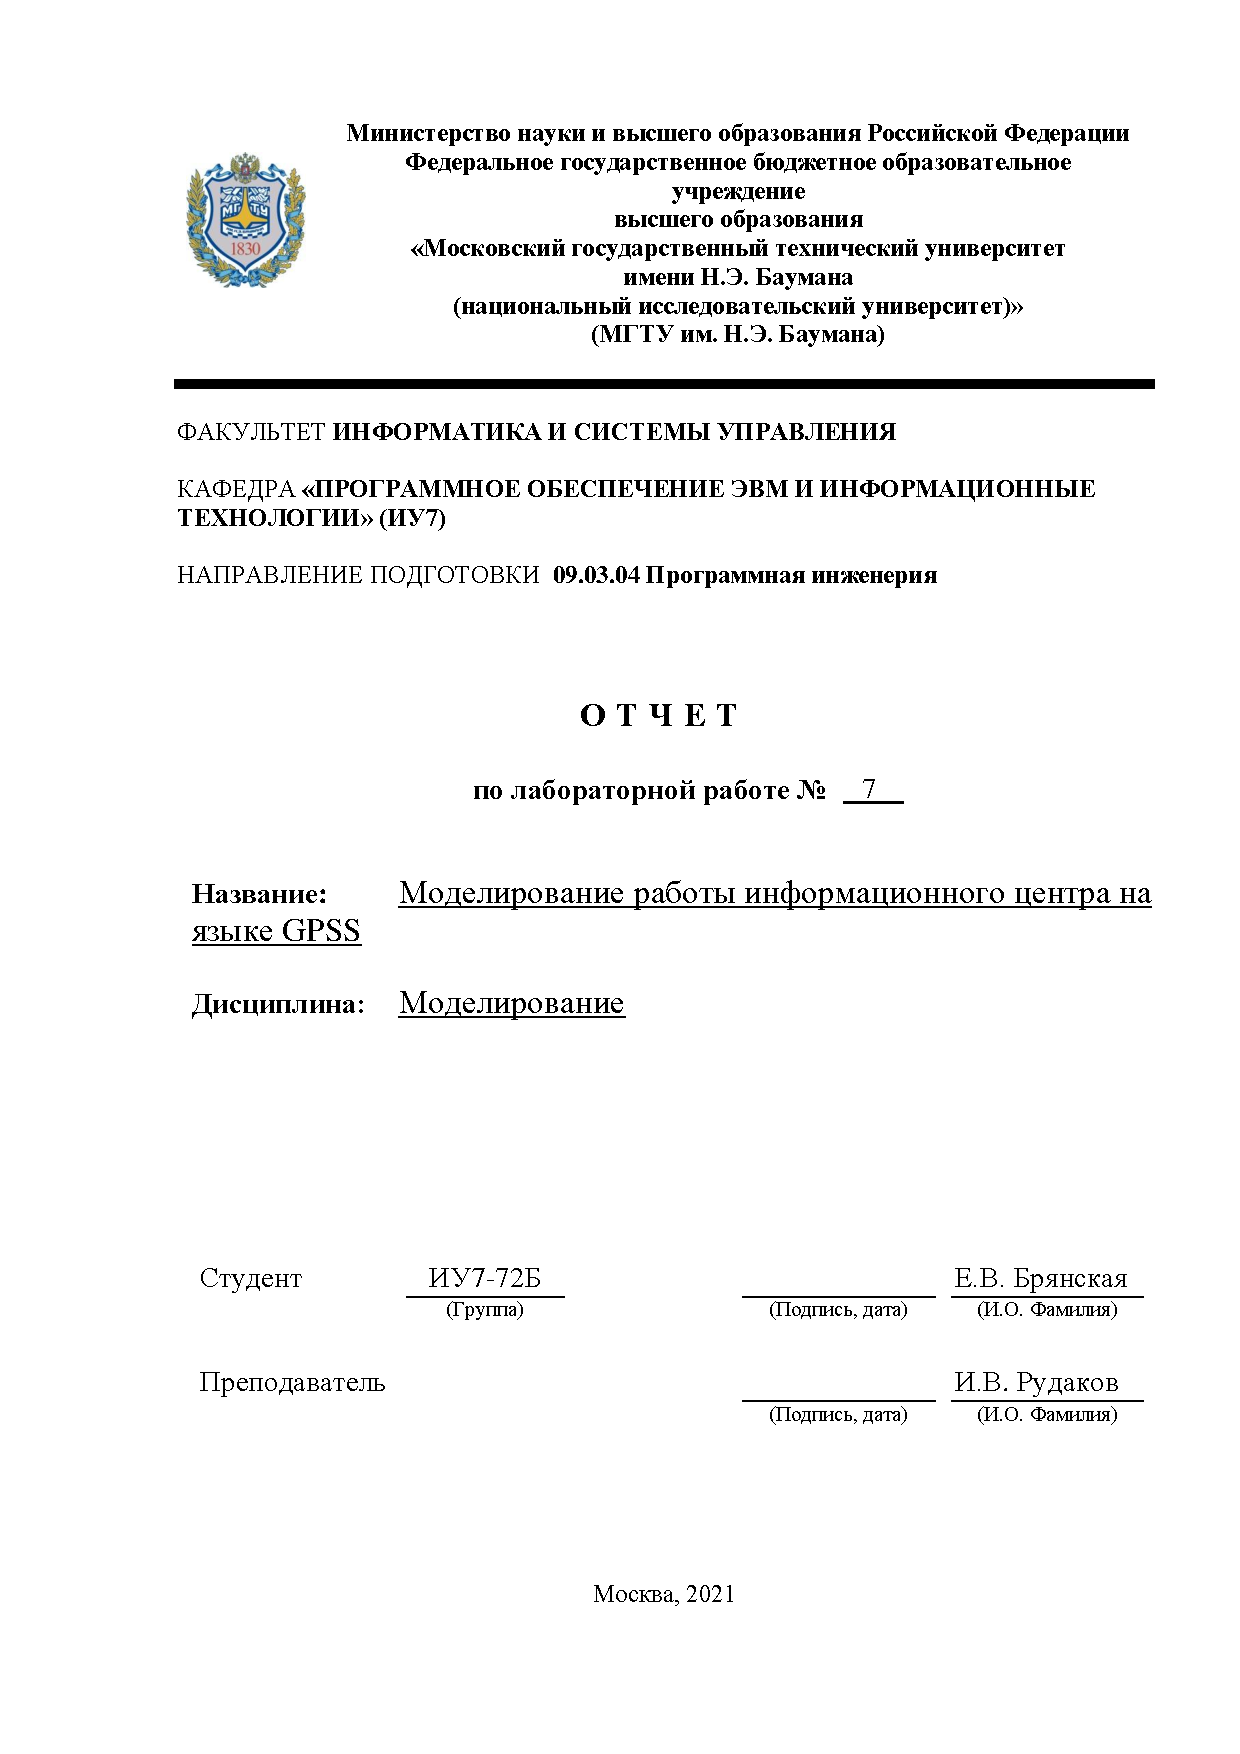
\includepdf[pages=1]{inc/title.pdf}
	
	%\tableofcontents
	%\newpage
	
	\section{Задание}
	В информационный центр приходят клиенты через интервал времени 10 $\pm$ 2 минуты. Если все три имеющихся оператора заняты, клиенту отказывают в обслуживании. 

Операторы имеют разную производительность и могут обеспечивать обслуживание среднего запроса пользователя за 20 $\pm$ 5; 40 $\pm$ 10; 40 $\pm$ 20. 

Клиенты стремятся занять свободного оператора с максимальной производительностью. 

Полученные запросы сдаются в накопитель. Откуда выбираются на обработку. На первый компьютер запросы от 1 и 2-ого операторов, на второй – запросы от 3-его. Время обработки запросов первым и 2-м компьютером равны соответственно 15 и 30 мин. Промоделировать процесс обработки 300 запросов.

Использовать язык GPSS.

\begin{figure}[h]
	\begin{center}
		{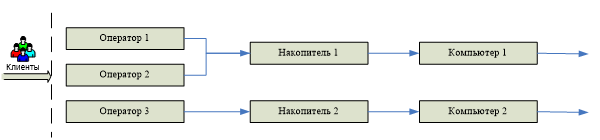
\includegraphics[scale = 0.9]{img/schema.png}}
		\caption{Общая схема}
		\label{fig1:image}
	\end{center}
\end{figure}
	%\newpage
	
	\section{Теоретическая часть}
	Существует три основных способа получения последовательностей случайных чисел:
\begin{enumerate}
	\item аппаратный;
	
	\item табличный (файловый);
	
	\item алгоритмический.
\end{enumerate}

В рамках лабораторной работы рассмотрены алгоритмический и табличный способы. 

\subsection{Алгоритмический способ}
Этот подход основан на базе специальных алгоритмов. К ним относятся:
\begin{itemize}
	\item метод серединных произведений;
	
	\item метод перемешивания;
	
	\item линейный конгруэнтный метод.
\end{itemize}

Было принято решение взять последний для генерации последовательности псевдослучайных чисел.

В этом методе каждое следующее число рассчитывается на основе предыдущего по формуле (\ref{formula1}).
\begin{equation}\label{formula1}
	R_{n + 1} = (a \cdot R_n + b)\;mod\;N,\, n \geq 1
\end{equation}
где a, b -- коэффициенты, N -- модуль.

Для качественного генератора требуется подобрать подходящие коэффициенты. Например, в таблице \ref{k} приведены некоторые из них.
\begin{table}[h]
	\begin{center}
		\caption{Примеры коэффициентов}
		\label{k}
		\begin{tabular}{| p{3cm} | p{3cm} | p{3cm}|}
			\hline
			\textbf{a} 			& \textbf{b} 	& \textbf{N} \\
			\hline
			106 				& 1283 			& 6075 \\ 
			\hline
			430 				& 2531  		& 11979 \\ 
			\hline
			84589 				& 15989 		& 217728 \\ 
			\hline
			1103515245 			& 12345 		& $2^{31}$ \\ 
			\hline
			... 				& ... 			& ... \\ 
			\hline
		\end{tabular}
	\end{center}
\end{table} 

\subsection{Табличный способ}
В качестве источника случайных чисел используют специально заранее составленные таблицы, содержащие проверенные данные.

\subsection{Критерий оценки}
В рамках лабораторной работы в качестве статистической оценки используется критерий <<хи-квадрат>> ($\chi^2$-критерий).

Привлекая этот критерий можно оценить, удовлетворяет ли генератор требованию равномерного распределения или нет.

Используется статистика, представленная формулой (\ref{formula2}).
\begin{equation}\label{formula2}
	V = \frac{1}{n}\sum_{s=min}^{max} \left( \frac{Y_s^2}{p_s} \right) - n
\end{equation}
где n - длина последовательности, min/max - границы, в пределах которых находятся элементы последовательности, $Y_s$ - число повторений числа s, $p = \dfrac{1}{max - min}$.

Вычисляется квантиль хи-квадрат от вычисленного V. Если полученное значение будет меньше 0.1 или больше 0.9, то эти числа считаются недостаточно случайными. Если же нет, то последовательность принимается как случайная. 

 
	\newpage
	
	\section{Результаты работы программы}
	Замеры проводились 10 раз, каждый раз моделировался процесс обработки 1000 клиентов. Проводился подсчёт обслуженный и отказанных заявок, времени моделирования и максимального размера очередей. Результаты приведены на рисунке \ref{fig3:image}.

\begin{figure}[h]
	\begin{center}
		{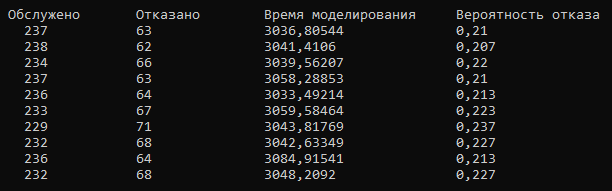
\includegraphics[scale = 0.75]{img/results.png}}
		\caption{Результаты моделирования}
		\label{fig3:image}
	\end{center}
\end{figure}
	\newpage
	
	
	\section{Код программы}
	На Листинге \ref{code} представлены основные методы.

\begin{lstlisting}[label=code, caption = Основные методы]
namespace lab05
{
	class ModelInfo
	{
		public Client clients;
		public Operator[] oprArr;
		public Computer[] comArr;
		public Queue<double> q1;
		public Queue<double> q2;
	}
	
	class Model : ModelInfo
	{
		private static int _goal;
		public int processed;
		public int refused;
		public double simTime;
		public double pRefuse;
		List<Event> eventArr;
		
		public Model(int goal)
		{
			processed = 0;
			refused = 0;
			q1 = new Queue<double>();
			q2 = new Queue<double>();
			eventArr = new List<Event>();
			
			clients = new Client(8, 12);
			comArr = new Computer[2]
			{
				new Computer(15, ref q1),
				new Computer(30, ref q2)
			};
			oprArr = new Operator[3]
			{
				new Operator(15, 25, ref q1),
				new Operator(30, 50, ref q1),
				new Operator(20, 60, ref q2)
			};
			
			_goal = goal;
		}
		
		public void Imitation()
		{
			Event curEvent;
			eventArr.Add(new Event(EventType.IsClient, clients.Next()));
			
			while (eventArr.Count > 0)
			{
				if (refused + processed >= _goal)
					break;
				
				curEvent = eventArr[0];
				eventArr.RemoveAt(0);
				
				if (curEvent.etype is EventType.IsClient)   ProcessClient(curEvent);
				else if (curEvent.etype is EventType.IsOperator)    ProcessOperator(curEvent);
				else    ProcessComputer(curEvent);
				
				eventArr.Sort((Event x, Event y) =>
					x.etime > y.etime
					? 1 : -1);
			}
			
			simTime = eventArr[0].etime;
			pRefuse = CountPRefuse();
		}
		
		private void ProcessClient(Event e)
		{
			int refuse = 1;
			for (int i = 0; i < oprArr.Length; i++)
				if (oprArr[i].IsFree())
				{
					eventArr.Add(new Event(EventType.IsOperator, oprArr[i].Next(e.etime), i));
					oprArr[i].SetBusy();
					refuse = 0;
					break;
				}
			refused += refuse;
			eventArr.Add(new Event(EventType.IsClient, clients.Next(e.etime)));
		}
		
		private void ProcessOperator(Event e)
		{
			int temp;
			oprArr[e.ind].AddToQueue(e.etime);
			temp = (e.ind == 2) ? 1 : 0;
			
			if (comArr[temp].IsFree())
			{
				eventArr.Add(new Event(EventType.IsComputer, e.etime, temp));
				processed -= 1;
			}
			
			oprArr[e.ind].SetFree();
			oprArr[e.ind].next = 0;
		}
		
		private void ProcessComputer(Event e)
		{
			double tempValue;
			tempValue = comArr[e.ind].GetFromQueue();
			if (tempValue > 0)
			{
				comArr[e.ind].SetBusy();
				eventArr.Add(new Event(EventType.IsComputer, comArr[e.ind].Next(e.etime), e.ind));
			}
			else
				comArr[e.ind].SetFree();
			processed += 1;
		}
		
		private double CountPRefuse() { return (double)refused / (refused + processed); }
	}

	class Obj : Generator
	{
		public bool _isFree;
		public double next;
		
		public Obj(double a, double b) : base(a, b)
		{
			SetFree();
			next = 0;
		}
		
		public double Next(double cur_time = 0)
		{
			next = cur_time + ProcessTime();
			return next;
		}
		
		public bool IsFree() { return _isFree; }
		public void SetFree() { _isFree = true; }
		public void SetBusy() { _isFree = false; }
		public virtual void AddToQueue(double elem) { throw new Exception(); }
		public virtual double GetFromQueue() { throw new Exception(); }
	}

	class Client : Obj	{ public Client(double a, double b) : base(a, b) {} }

	class Computer : Obj
	{
		private Queue<double> _q;
		public Computer(double a, ref Queue<double> q) : base(a, a) { _q = q; }
		public override double GetFromQueue()
		{
			if (_q.Count != 0)
			return _q.Dequeue();
			return -1;
		}
	}

	class Operator : Obj
	{
		private Queue<double> _q;
		public Operator(double a, double b, ref Queue<double> q) : base(a, b) { _q = q; }
		public override void AddToQueue(double elem) { _q.Enqueue(elem); }
	}

	public enum EventType
	{
		IsClient,
		IsOperator,
		IsComputer
	}
	
	class Event
	{
		public EventType etype;
		public double etime;
		public int ind;
		public Event(EventType type, double time, int index = 0)
		{
			etype = type;
			etime = time;
			ind = index;
		}
	}

	class Generator
	{
		private double _a;
		private double _b;
		private Random rnd;
		public Generator(double a, double b)
		{
			_a = a;
			_b = b;
			rnd = new Random();
		}
		
		public double ProcessTime() { return _a + (_b - _a) * rnd.NextDouble(); }
	}
}

\end{lstlisting}
	
\end{document}
